%%
%% This is the sigconf entry point supplied by the ACM template package.
%% The sample article body has been replaced with the Joggle manuscript.
%%
%% Commands for TeXCount
%TC:macro \cite [option:text,text]
%TC:macro \citep [option:text,text]
%TC:macro \citet [option:text,text]
%TC:envir table 0 1
%TC:envir table* 0 1
%TC:envir tabular [ignore] word
%TC:envir displaymath 0 word
%TC:envir math 0 word
%TC:envir comment 0 0
%%
%% Anonymous two-column submission layout at the EuroSys minimum type size.
\documentclass[sigconf,anonymous,10pt]{acmart}

%% Balance the reference columns explicitly; acmart's end hook runs too late
%% once the bibliography has already entered the second column.
\makeatletter
\@ACM@balancefalse
\makeatother

\AtBeginDocument{%
  \providecommand\BibTeX{{%
    Bib\TeX}}}

\usepackage{algorithm}
\usepackage{algpseudocode}
\usepackage{amsmath}
\usepackage{balance}
\usepackage{listings}
\usepackage{xcolor}

%% Rights information is replaced by the ACM rights-form block for publication.
\setcopyright{none}
\copyrightyear{2027}
\acmYear{2027}
\acmConference[EuroSys '27]{EuroSys 2027}{April 19--23, 2027}{Rabat, Morocco}
\acmISBN{}
\acmDOI{}

\definecolor{jogblue}{HTML}{0B6FB8}
\definecolor{joggreen}{HTML}{147D64}
\definecolor{joggray}{HTML}{F4F6F8}
\definecolor{jogcomment}{HTML}{667085}

\lstdefinelanguage{jog}{
  sensitive=true,
  morekeywords={mod,use,fn,local,let,var,if,else,for,in,return,true,false},
  morecomment=[l]{//},
  morestring=[b]"
}

\lstset{
  basicstyle=\ttfamily\scriptsize,
  keywordstyle=\color{jogblue}\bfseries,
  commentstyle=\color{jogcomment},
  stringstyle=\color{joggreen},
  backgroundcolor=\color{joggray},
  frame=single,
  rulecolor=\color{black!12},
  framesep=4pt,
  xleftmargin=3pt,
  xrightmargin=3pt,
  breaklines=true,
  breakatwhitespace=false,
  columns=fullflexible,
  keepspaces=true,
  showstringspaces=false,
  captionpos=t
}

\begin{document}

\title[Joggle]{Joggle: Malleable Compilation with a Progressive Intermediate Representation}

\begin{abstract}
Extending a heterogeneous compiler is a cross-cutting task. One feature can
require a semantic definition, an analysis, a graph transformation, a
conversion, and an artifact generator, yet established infrastructures expose
these roles through different extension and invalidation mechanisms. Joggle
makes compiler behavior part of the program model. Programs and compiler
extensions share one typed graph, one function language, and one value model;
graph-level \emph{mods} define ownership and dependency boundaries across
stages; and an evaluator records graph observations and effects while
publishing updates transactionally. The resulting intermediate representation
is progressive: typed compiler functions refine verified mods without
requiring a fixed sequence of public IR classes. Joggle combines stable graph
handles, hierarchical revisions, dependency indices, and cached execution
plans to re-execute only stages whose recorded inputs may have changed. We
evaluate the design through held-out compiler-extension tasks, matched
cross-system feature patches, controlled edits over a pinned full-model corpus,
and operator- and model-level artifact measurements. The evidence tests whether
extensions are predictable to generate, whether changes remain within their
ownership boundary, and whether update cost follows the affected graph rather
than the complete pipeline.
\end{abstract}

\keywords{compilers, extensibility, metaprogramming, incremental compilation}

\ccsdesc[500]{Software and its engineering~Compilers}

\maketitle

\section{Introduction}
\label{sec:introduction}

Compilers for heterogeneous systems coordinate decisions at several scales.
They define operator semantics, transform graphs, schedule loops and memory,
convert representations, and generate artifacts for processors and
accelerators. LLVM established the value of a shared typed representation for
analysis and transformation~\cite{lattner2004llvm}; MLIR generalized this
approach to multiple abstraction levels~\cite{lattner2021mlir}; Halide
separated algorithms from schedules~\cite{ragankelley2012halide}; and TVM
combined graph- and operator-level optimization for diverse
targets~\cite{chen2018tvm}. Together they make programs increasingly malleable,
but the compiler's own extension model remains divided among mechanisms with
different syntax, ownership, and execution rules.

Consider adding a numeric format or a target-specific operator family. Its
semantic definition may live in an operator registry, legality in an analysis,
selection in a pass, representation changes in conversions, and realization in
an emitter or runtime binding. Each mechanism is individually useful, yet the
extension is the conjunction of all of them. A developer must reconstruct the
cross-layer contract before making a local change. A code-generating agent
faces the same structural burden: a plausible edit can omit a registration
path, modify the wrong representation, or trigger a wider rebuild and rerun
than the change requires.

This fragmentation creates three coupled problems. First, compiler behavior is
expressed through several extension interfaces, so one logical feature cannot
be inspected or generated through one language. Second, ownership follows
source trees, registries, and IR layers instead of the feature's dependency
boundary, so its change surface grows with the compiler. Third, staged drivers
usually track whole pass results, so a small edit can repeat conversions and
analyses whose observations remain valid. These are programmability,
organization, and update-efficiency problems, respectively.

Figure~\ref{fig:thesis-map} states the paper's argument as three vertical
chains. Each column connects a development problem to one Joggle mechanism and
one measurable outcome. This 3$\times$3 mapping also aligns the evaluation with
the design: held-out extension tasks measure predictability and executable
completion, paired patches measure change footprint, and controlled edits
measure update latency and executed work.

\begin{figure*}[t]
  \centering
  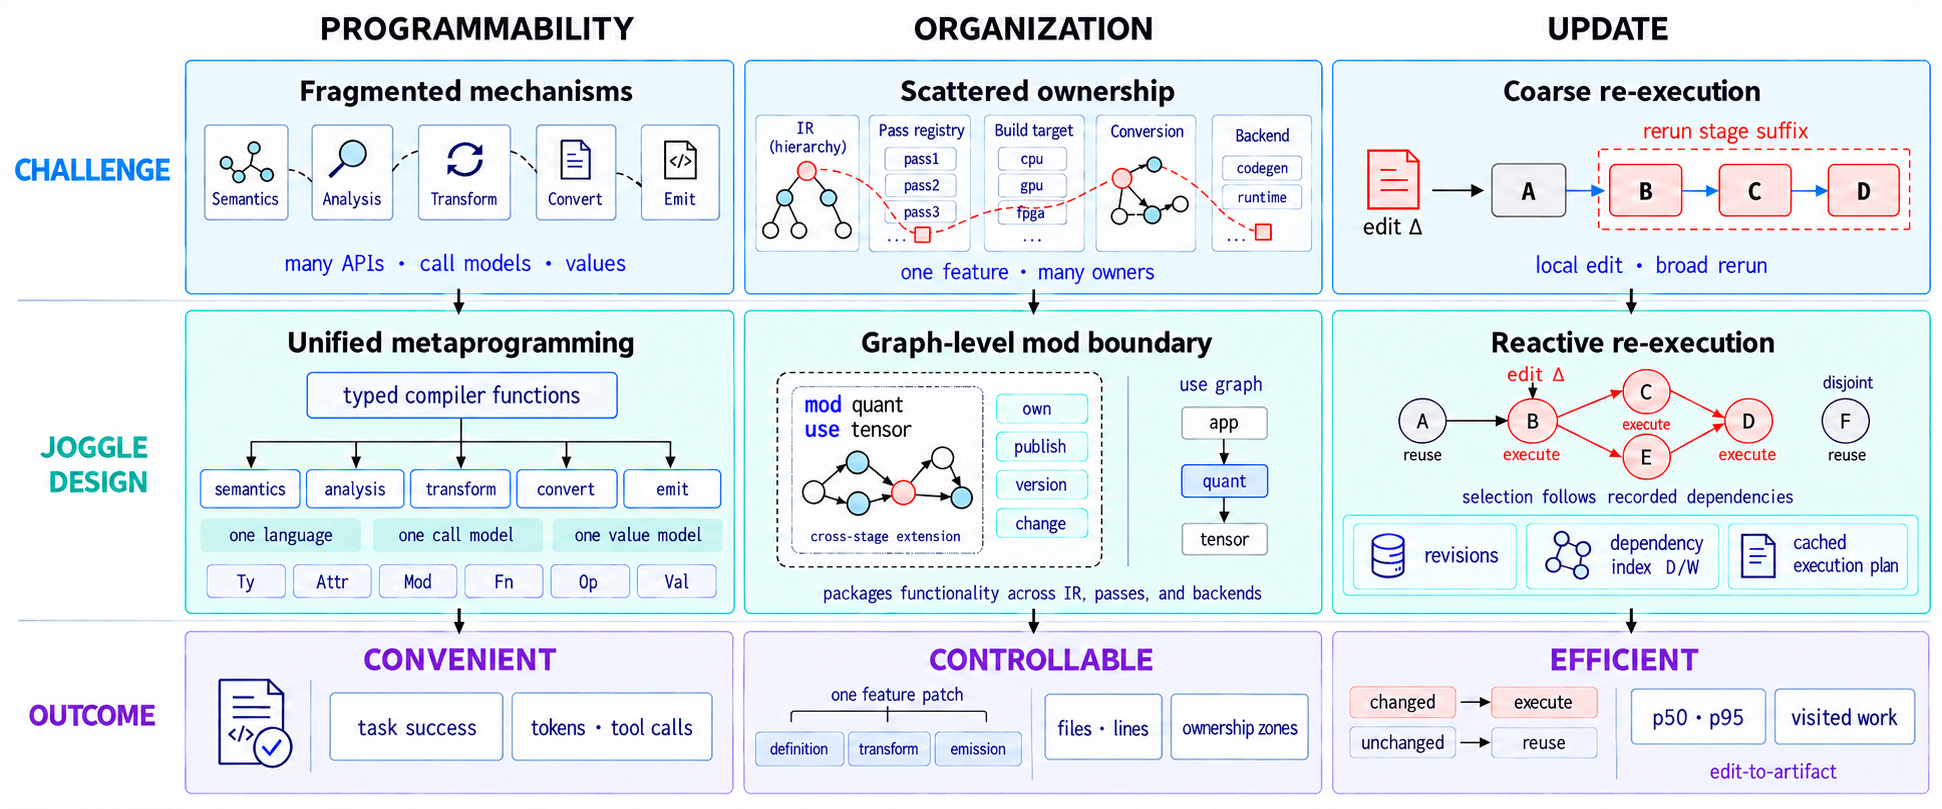
\includegraphics[width=.94\textwidth]{figures/figure-01-thesis-map.png}
  \caption{Joggle maps three extension challenges to system mechanisms and
    measurable outcomes.}
  \Description{A three-column, three-row argument map read top to bottom.
    Fragmented mechanisms map to unified metaprogramming and convenient
    extension. Scattered ownership maps to a graph-level mod boundary and
    controllable change. Coarse re-execution maps to revisions, dependency
    indices, cached plans, and efficient updates.}
  \label{fig:thesis-map}
\end{figure*}

Joggle addresses these problems by making compiler behavior part of the
program model. A Joggle program and its compiler extensions use the same typed
graph and the same function language. Analyses, transformations, converters,
and artifact generators are ordinary typed \emph{compiler functions}. A
\emph{mod} owns such functions with its graph, native bindings, and explicit
\texttt{use} dependencies. An evaluator executes calls transactionally,
observes the graph state they read, and records the effects they publish.

We call the representation \emph{progressive} because compilation proceeds
through typed refinements of one verified graph. A mod may retain semantic
operations, introduce lower-level
helpers, or replace selected definitions; each published intermediate remains
an inspectable Joggle mod. Progress is therefore chosen by typed functions and
explicit dependencies, not encoded as a mandatory global pipeline.

This design yields three contributions.

\paragraph{Unified metaprogramming.}
One language, call model, and value model cover semantic definitions, analyses,
graph transformations, representation conversion, and artifact generation
while retaining distinct read and write contracts.

\paragraph{Mod-scoped composition.}
Graph-level mod packages define ownership, publication, dependency, and change
boundaries across compilation stages. This boundary is orthogonal to
hierarchical program IR.

\paragraph{Dependency-directed updates.}
Revisions, dependency indices, and cached execution plans restrict
re-execution to compiler calls and stages whose recorded observations overlap
published edits, under transactional publication.

The evaluation assigns one evidence stream to each contribution. Held-out
extensions measure predictability and executable task success. Matched feature
patches measure repository footprint. Controlled edits over complete models
measure latency and executed work. Artifact quality and mechanism costs
complete the evidence chain while reporting compiler responsiveness and
generated-code quality separately.

\section{Motivation and Design Requirements}
\label{sec:motivation}

\subsection{Compiler Extension Workflow}
\label{sec:workflow}

Figure~\ref{fig:workflow} summarizes where extension work enters a
heterogeneous compilation stack. Model formats carry structures and semantics
into the compiler. Operator-level transformations specialize individual
computations; graph-level transformations fuse, propagate, or quantize across
operations; system-level transformations plan ordering, storage, and
communication. The runtime then supplies execution and platform support before
deployment to a target. These levels cooperate, but they are commonly exposed
through different APIs and maintained by different developers.

\begin{figure}[t]
  \centering
  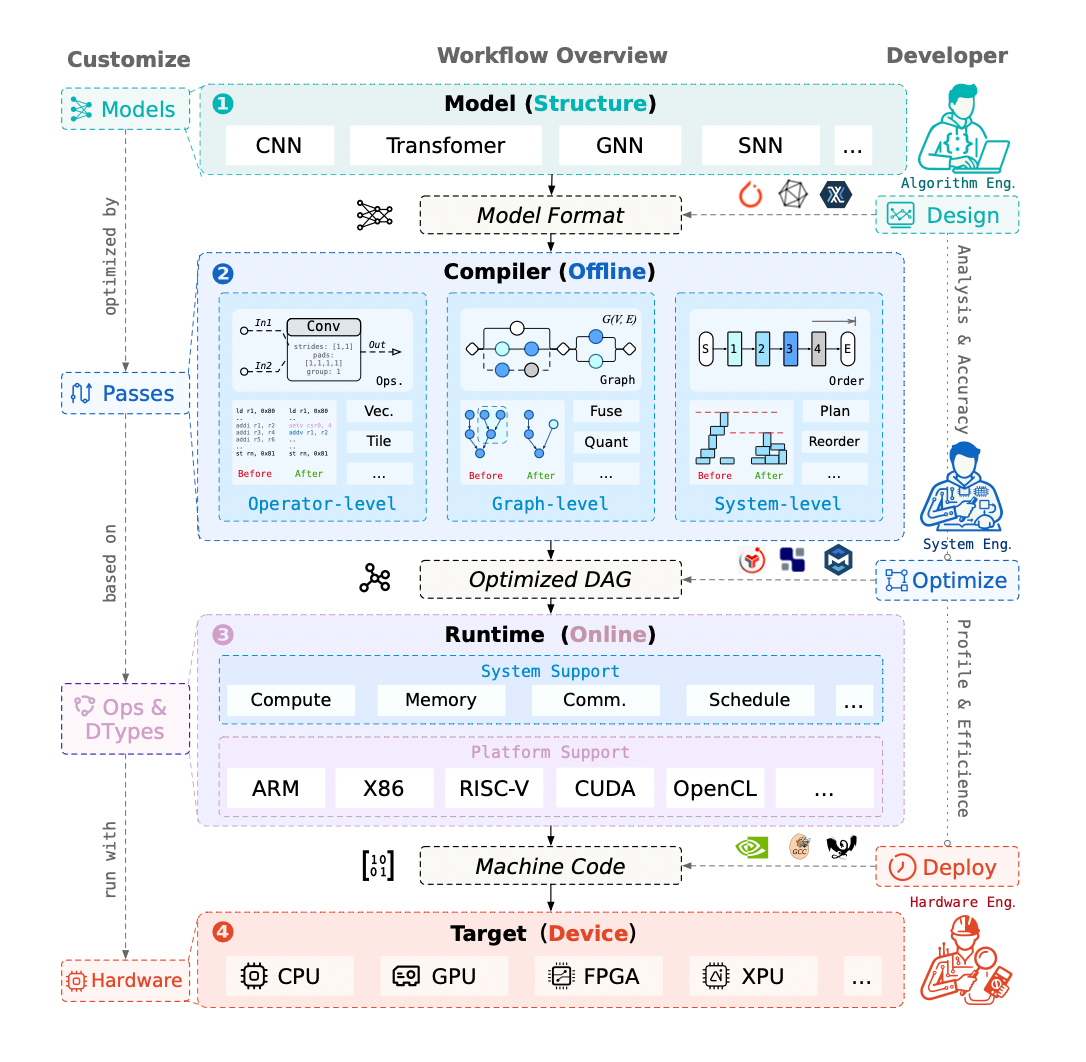
\includegraphics[width=\columnwidth]{figures/figure-02-workflow.png}
  \caption{A compiler extension can span semantic definition, optimization,
    runtime support, and target deployment.}
  \Description{A workflow from model structure and model formats through
    operator-, graph-, and system-level compilation, an online runtime, and
    target devices. The sides show customization artifacts and the algorithm,
    system, and hardware developers who create them.}
  \label{fig:workflow}
\end{figure}

Consider adding a fused convolution, bias addition, and activation. The
extension defines the fused operator's semantics, checks shapes and uses,
replaces a matching subgraph, selects a target implementation, and emits an
artifact. These responsibilities span several stages in
Figure~\ref{fig:workflow}. A later change to the supported layout or numeric
type must preserve agreement among the legality test, transformation, and
target implementation. Section~\ref{sec:design} uses this operator extension
to make the interfaces and ownership boundary concrete.

Existing infrastructures offer rich extension points for these individual
roles. The difficulty addressed here is their composition: a complete feature
must connect declarations, transformations, target realization, and
invalidation even when those roles have separate interfaces and ownership
boundaries.

\subsection{Development Friction}
\label{sec:friction}

\paragraph{Fragmented metaprogramming.}
An operator schema describes admissible programs, but a pass, converter, and
emitter describe actions over those programs. When each role uses a different
registration and invocation model, neither a person nor a synthesis tool can
treat the feature as one typed program. The required context includes framework
conventions that are absent from the local definition, increasing both
implementation effort and the opportunity for an incomplete extension.

\paragraph{Diffuse ownership.}
Hierarchical IRs organize operations inside regions, blocks, and functions.
That containment expresses program semantics; compiler capabilities
additionally need ownership and dependency boundaries. Capability ownership is
often reconstructed from directories, build
targets, registries, and pass ordering. A feature revision can therefore touch
files and subsystems outside its semantic boundary, making review, replacement,
and parallel development harder to control.

\paragraph{Coarse update boundaries.}
A conventional pipeline establishes correctness by running an ordered sequence
of stages over each new input. After a local graph or policy edit, rerunning the
affected suffix is safe but can be unnecessarily broad: an analysis that did
not observe the edited entity is recomputed, and a later stage can be rerun even
when an earlier stage publishes no relevant effect. Materialized representation
boundaries add further units to rebuild, validate, and traverse.

The three costs reinforce one another. Fragmented interfaces spread a feature;
spread ownership enlarges its change surface; a larger change surface forces
coarser invalidation. Addressing only one layer leaves the other two as limits
on extension velocity.

\subsection{Design Requirements}
\label{sec:requirements}

The preceding workflow gives three requirements for a malleable compiler.

\paragraph{R1---One typed extension surface.}
Semantic definitions, analyses, transformations, converters, and artifact
generators must share one language, call model, and value model. The surface
preserves explicit effects: read-only queries and mutating transformations use
distinct publication rules within the same syntax.

\paragraph{R2---Explicit capability composition.}
A feature must have a named owner, public and private functions, declared
dependencies, and an independent lifecycle. This graph-level package boundary
is orthogonal to hierarchical program containment, making a compiler capability
installable, inspectable, replaceable, and removable through its owner.

\paragraph{R3---Change-proportional execution.}
Revisions and dependency indices must validate the state a function actually
observed and propagate only effects that can reach a later observation. Cached
execution plans must avoid repeated setup. Updates remain transactional:
records and plans become reusable only with the verified graph from which they
were derived.

These requirements determine Joggle's structure. Compiler functions provide
R1, mods provide R2, and the evaluator and graph runtime provide R3. The next
section develops these mechanisms in the order in which a call uses them.

\section{Joggle Design}
\label{sec:design}

\subsection{System Model}
\label{sec:system-model}

Joggle represents programs and compiler extensions with the same typed graph
substrate. A \emph{subject mod} contains the program being inspected or
changed, whereas an \emph{extension mod} contributes compiler functions. Both
are ordinary mods: they use the same graph representation, type system,
dependency rules, and loader. The distinction describes their role in one
invocation, not two different runtime objects.

The graph owned by a mod is
\[
  G = (F, B, O, V, A),
\]
where $F$, $B$, $O$, and $V$ are functions, blocks, operations, and values, and
$A$ denotes attributes attached to these entities. Blocks order operations,
operations consume and produce values, and maintained def--use edges connect
each value to its users. Operator sets, input formats, and artifacts enter
through extension mods.

An environment $E$ loads the mods named by a program, resolves typed calls,
binds source or native implementations, and owns evaluator state. One
compiler-function call has the form
\[
  E \vdash f(M, a) \Downarrow (r, D, W).
\]
Here, $M$ is the subject mod and $a$ contains explicit arguments. The call
returns $r$, records the observed graph state $D$, and publishes graph effects
$W$. Read-only calls have $W=\varnothing$. Mutating calls produce $W$ only
after the resulting graph passes verification.

Joggle calls this representation progressive because each successful compiler
function publishes another verified mod over the same entity model. A stage may
retain semantic operations while introducing lower-level helpers, and a later
stage may replace definitions it owns. Typed refinements express progress
within one graph model, and every published state remains inspectable.

The rest of the design follows the three requirements from
Section~\ref{sec:requirements}. Section~\ref{sec:compiler-functions} realizes
R1 with typed compiler functions. Section~\ref{sec:mods} realizes R2 with
mod-scoped composition. Sections~\ref{sec:incremental}
and~\ref{sec:graph-runtime} realize R3 through observed dependencies and the
graph runtime that validates them.

\subsection{Compiler Functions}
\label{sec:compiler-functions}

Joggle's metaprogramming interface is the typed compiler function. Operator
semantics, analyses, transformations, representation conversion, and artifact
generation use this single programmable surface for definition and invocation.

A compiler function accepts graph handles and ordinary values:
\[
  f : (H_1, \ldots, H_n, A_1, \ldots, A_m) \rightarrow R.
\]
Each $H_i$ is a \texttt{Mod}, \texttt{Fn}, \texttt{Blk}, \texttt{Op}, or
\texttt{Val} handle. Each $A_i$ is a configuration or structural value, such
as an integer, type, list, dictionary, or \texttt{Attr}. The result $R$ may
itself be a handle, an ordinary value, structured data, text, or bytes. Handles
retain graph ownership and lifetime; ordinary values remain independent of
graph storage.

A common operator extension illustrates these roles in
Figure~\ref{fig:operator-extension}. A convolution, bias addition, and
activation form a fusible subgraph. One mod owns the fused
operator's semantic contract together with typed functions for legality
analysis, fusion, target conversion, and artifact generation. The functions
exchange graph handles and owned values through the interface above; each role
retains its own effect contract.

\begin{figure}[t]
  \centering
  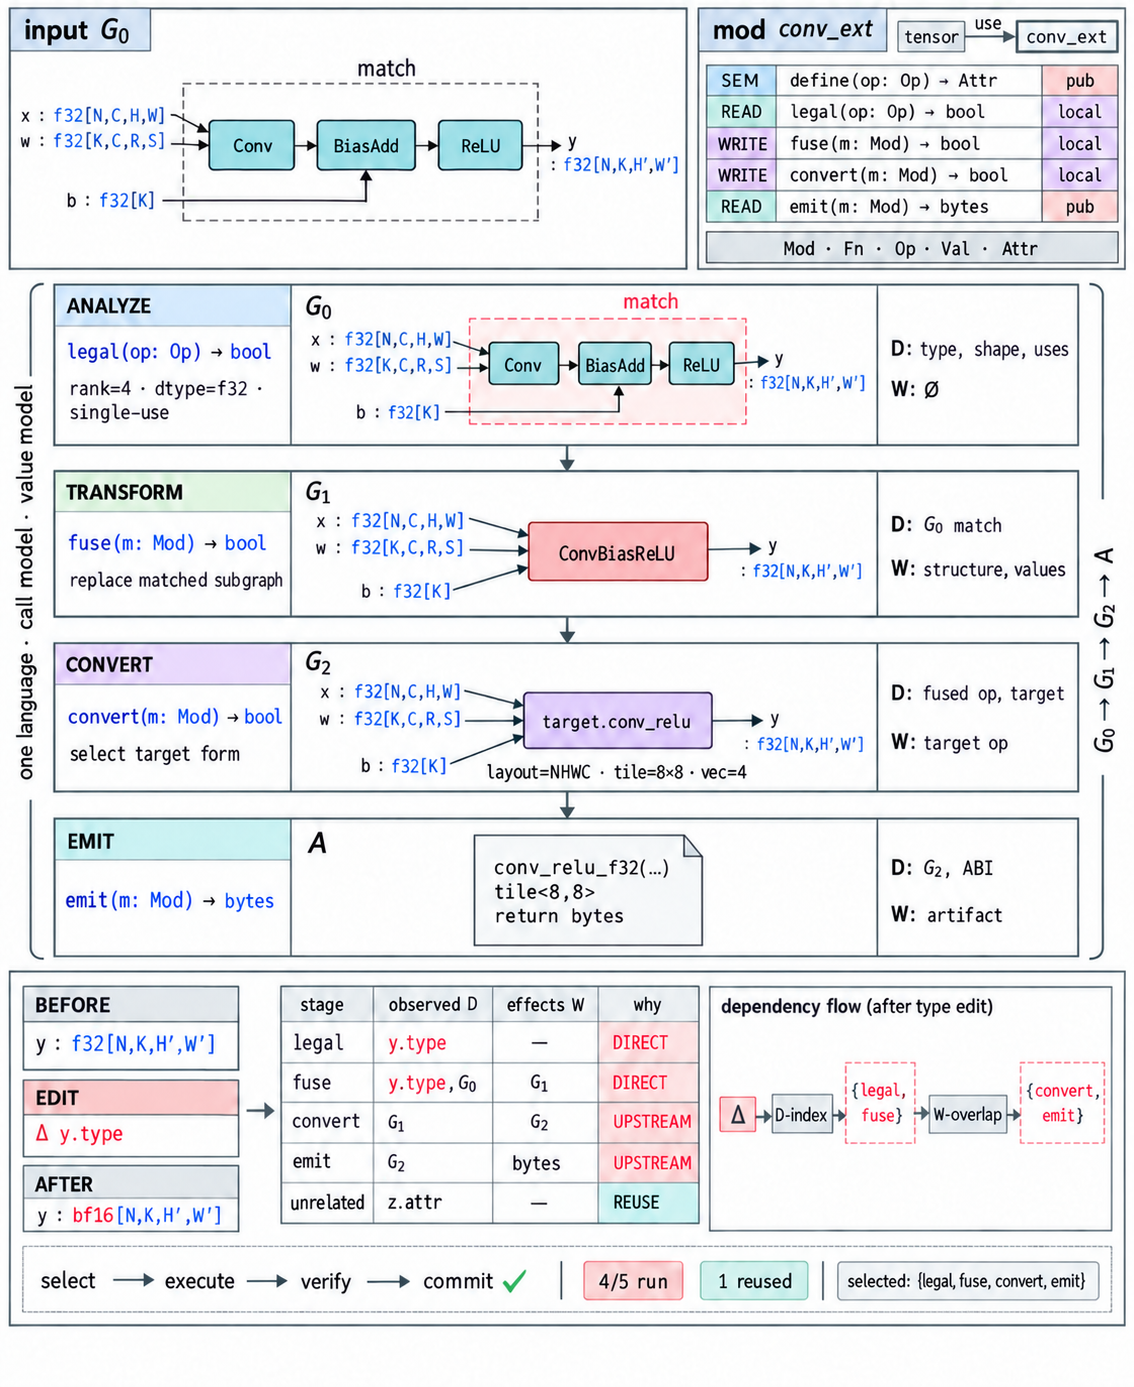
\includegraphics[width=\columnwidth]{figures/figure-03-operator-extension.png}
  \caption{One operator extension in Joggle. Five compiler roles share typed
  calls; recorded observations and effects select work after a local edit.}
  \Description{A typed convolution, bias, and activation graph is analyzed,
  fused, converted to a target operation, and emitted by five functions in one
  mod. The graph progresses through three verified states to an artifact. A
  type edit directly selects legality and fusion, propagates through conversion
  and emission, reuses an unrelated analysis, and commits transactionally.}
  \label{fig:operator-extension}
\end{figure}

Joggle resolves a call from its qualified name, visible mods, explicit generic
arguments, parameter types, and result context. The selected implementation may
be a source body, an intrinsic, or a native binding. Caller syntax and the
evaluator's result boundary remain identical across these implementations.

Uniform calls retain distinct effect contracts. A query evaluates against a
read-only mod and returns an \texttt{Attr}. A run applies one or more mutating
functions within a transaction. An artifact call evaluates read-only over a
prepared graph and returns text or bytes. Thus, \texttt{query}, \texttt{run},
and \texttt{emit} share resolution and evaluation while preserving different
publication rules. Read-only execution rejects mutation, and a run publishes
only a verified graph.

Compiler functions also compose through ordinary calls. A fusion function can
invoke its legality analysis, and a conversion can query the fused operator's
semantic contract. These calls remain visible to type checking, diagnostics,
and dependency capture. The typed call graph therefore defines composition
directly.

This function model unifies how compiler behavior is declared, resolved, and
invoked. Mods then supply the namespace, visibility, and dependency boundaries
that organize these functions.

\subsection{Mods}
\label{sec:mods}

A mod is Joggle's unit of ownership and composition. We model it as
\[
  \mathcal{M} = (n, U, F_{\mathrm{pub}}, F_{\mathrm{local}}, G, N).
\]
where $n$ is the mod name and $U$ is its declared \texttt{use} set.
$F_{\mathrm{pub}}$ and $F_{\mathrm{local}}$ are its public and local
functions, $G$ is its graph, and $N$ contains optional native bindings. The
loaded object is the semantic boundary; its on-disk package is the distribution
form.

The \texttt{use} declarations form a directed mod graph. Search roots determine
where a named mod can be found, while \texttt{use} edges select the dependencies
that participate in loading and resolution. Separating location from dependency
keeps neighboring installations outside the visible function set.

Loading validates the declared dependency closure before evaluation. The loader
rejects missing mods, cycles, declaration-name mismatches, duplicate public
signatures, unreadable fragments, and unresolved native bindings. It then loads
source fragments in deterministic order. For a fixed mod graph and search-root
order, this process yields a stable public function set.

Visibility keeps this public set small. A public function can be resolved by a
dependent mod, whereas a \texttt{local fn} remains inside its owner. Source
fragments may split a large implementation without creating new dependency or
lifecycle boundaries. A separate mod is appropriate when a capability needs an
independent public surface, dependency set, owner, or installation lifecycle.

Native code follows the same boundary. A body-less declaration names the typed
contract, and a native library owned by that mod supplies its implementation.
The binding is scoped to the owning mod and becomes available through the
declared dependency graph.

Lifecycle operations preserve the same closure. Installation stages a
candidate, loads and verifies its dependencies, and publishes it only after
validation succeeds. Upgrade additionally checks affected reverse dependencies.
A failed operation leaves the installed graph unchanged. These rules make the
mod the unit that evolves across installation and upgrade.

The mod graph is orthogonal to the containment structure inside a subject
program. Blocks and operations describe program structure; \texttt{use} edges
describe compiler capability. The former may change during transformation
without rewriting the latter. This separation lets one project compose
analysis, transformation, and artifact mods without embedding those ownership
decisions into its program IR.

Static mod dependencies state what a compiler extension may call. During
execution, the evaluator records which functions and
graph entities a call actually observes. Section~\ref{sec:incremental} uses this
second, dynamic dependency graph to avoid re-executing unaffected work.

\subsection{Incremental Evaluation}
\label{sec:incremental}

A local graph edit need not invalidate every compiler result. Joggle bases reuse
on observed state rather than on the subject mod's whole revision alone. For a
cached read-only call $c$, the evaluator stores
\[
  C_c = (K_c, r_c, D_c),
\]
where $K_c$ identifies the environment, store, function, and arguments; $r_c$
is the returned value; and $D_c$ contains the observations made while computing
it.

Observations follow the graph API used by the function. Reading one operation
records its identity, generation, and payload state. Reading one value also
records type, metadata, and def--use state. Traversing a function records the
relevant function revision or collection membership. Reading all operations,
the mod structure, or the \texttt{use} set records progressively broader state.
The evaluator therefore captures the narrowest observation that preserves the
semantics of each graph operation.

Range access records the structural revision together with only the returned
operations. A content edit outside the range therefore preserves the record,
whereas insertion, removal, or reordering invalidates its structural premise.

A cached query is reusable when its call key and every recorded observation
remain current:
\[
  \operatorname{Reusable}(c) = \operatorname{Same}(K_c) \land
  \bigwedge_{d \in D_c} \operatorname{Current}(d).
\]
On a hit, the evaluator returns $r_c$. On a miss, it evaluates the function in
read-only mode, captures a fresh $D_c$, and replaces the entry. The execution
report names the first invalid contract, such as an environment, structure,
function, operation, or value change. Generation checks distinguish an edited
entity from a new entity that later reuses the same slot.

Mutating pipelines require one further step. After a successful run, a reactive
schedule stores for each stage $s_i$ its call key $K_i$, observed inputs $D_i$,
and output scope $W_i$. The key names the environment, function, and arguments.
The output scope contains changed function identities and flags for structural
or mod-dependency changes. On the next run, a stage is selected when its key or
inputs are stale, or when an earlier selected stage may change something it
observed:
\[
  \begin{aligned}
    \operatorname{Selected}_i ={}&
      \neg \operatorname{Current}(K_i,D_i) \\
      &\lor \exists j<i:\ \operatorname{Selected}_j \land
      \operatorname{Overlap}(W_j,D_i).
  \end{aligned}
\]
The second term is an \emph{upstream} miss. The inputs recorded for $s_i$ may
still match at the start of a run, yet an earlier stage selected in the same run
can change them. Propagating recorded output scopes restricts downstream
selection to overlapping regions instead of forcing all later stages to execute.

\begin{algorithm}[t]
  \caption{Reactive stage selection and execution}
  \label{alg:reactive}
  \begin{algorithmic}[1]
    \State $dirty \gets \varnothing$; $selected \gets \varnothing$
    \For{each stage $s_i$ in schedule order}
      \State $miss \gets \operatorname{validate}(K_i,D_i)$
      \If{$miss=\varnothing \land \operatorname{overlap}(dirty,D_i)$}
        \State $miss \gets \mathrm{upstream}$
      \EndIf
      \If{$miss\neq\varnothing$}
        \State $selected \gets selected \cup \{s_i\}$
        \State $dirty \gets dirty \cup W_i$
      \EndIf
    \EndFor
    \State begin transaction
    \For{each $s_i\in selected$ in schedule order}
      \State execute $s_i$ and capture fresh $D_i,W_i$
    \EndFor
    \State verify and commit graph
    \State replace selected records and rebase retained records
    \State publish all records for the next run
  \end{algorithmic}
\end{algorithm}

Dependency records are published only after all selected stages execute and the
final graph verifies. Failure rolls back graph mutations and revision state; it
also discards the tentative records. Consequently, the next run cannot reuse
dependencies derived from an unpublished graph.

In Figure~\ref{fig:operator-extension}, a type edit directly invalidates the
legality and fusion stages that observed it. Because fusion may replace the
matched subgraph, conversion is selected by overlap with that potential
effect; artifact generation follows conversion for the same reason. An
analysis with disjoint observations retains its previous result.

Fine-grained observations reduce re-execution but add capture and validation
work. For $K$ stages, incremental latency is approximately
\[
  \begin{aligned}
    T_{\mathrm{select}}
      &= \sum_{i=1}^{K} T_{\mathrm{validate}}(K_i,D_i)
         + T_{\mathrm{propagate}}, \\
    T_{\mathrm{inc}}
      &= T_{\mathrm{select}}
         + \sum_{s_i \in \mathrm{Selected}} T_{\mathrm{eval}}(s_i) \\
      &\quad + T_{\mathrm{verify}}(G') + T_{\mathrm{commit}}.
  \end{aligned}
\]
Reuse is beneficial when this cost is lower than executing the omitted stages.
Broad graph APIs remain correct but record broad dependencies; narrow APIs can
preserve results across unrelated edits. External mutable state must enter
through typed arguments or an environment change before reuse. Native bindings
exchange scalar or byte attributes and do not receive graph entities, so
graph-dependent work remains in tracked compiler functions. These rules define
the state over which Joggle can validate reuse.

Incremental evaluation therefore depends on more than a result cache. It
requires stable entity identity, revisions that reflect every published edit,
and transactions that align graph state with dependency state. The graph
runtime provides these mechanisms.

\subsection{Graph Runtime}
\label{sec:graph-runtime}

Each mod owns a store with separate slot arrays for functions, blocks,
operations, and values. Public graph entities are small handles
\[
  h = (S, i, g),
\]
where $S$ identifies the store, $i$ selects a slot, and $g$ is that slot's
generation. A lookup succeeds only when the store matches and the slot is live
at generation $g$. Erasing an entity advances its generation, so a stale handle
cannot refer to a later entity that reuses the same slot.

The store maintains whole-mod, structural, and function revisions. Any
observable edit advances the whole revision. Membership, order, and topology
changes also advance the structural revision, while function-local changes
advance the owning function's revision. These counters serve as freshness
tokens. Their granularity lets a function-level
observation survive an unrelated edit elsewhere in the mod.

Graph relations are updated with the store. In particular, each value records
its users. Replacing a value can therefore walk the affected uses, update both
def--use lists, and touch the owning functions without scanning every operation.
Repeated affected-cone walks use epoch marks, avoiding a graph-sized bitmap
clear before each sparse traversal.

Mutations execute inside a transaction. Metadata edits journal the previous
leaf value. Structural edits acquire a store snapshot lazily, when the first
such edit occurs. After evaluation, the verifier checks ownership, liveness,
dominance, calls, block arguments, return types, and structured control flow.
The publication rule is
\[
  \operatorname{Publish}(f,G) =
  \begin{cases}
    (G', \mathrm{ok}) &
      \text{if } f:G \Downarrow G'
      \land \operatorname{Verify}(G'), \\
    (G, \mathrm{fail}) & \text{otherwise.}
  \end{cases}
\]
Verification therefore prevents a locally valid edit from exposing a globally
invalid graph. Success commits the graph and its revisions; failure restores
both.

The evaluator uses predecoded plans for checked compiler functions. A plan maps
parameters, block arguments, and operation results to dense slots; it
also records block targets, operation kinds, operand indices, and call-site
information. Its cache key is
\[
  \operatorname{PlanKey} =
  (S, \operatorname{id}(fn), \operatorname{generation}(fn),
   \operatorname{revision}(fn)).
\]
Changing a function body invalidates its plan, while calls to the same version
reuse decoding and slot layout. Stable call sites additionally cache overload
resolution under the current environment epoch and argument types. Reusable
register windows reduce per-call allocation.

These plans are an internal interpreted execution form. They remove repeated
decoding and slot-allocation setup while preserving the language's control
flow, failure propagation, and dynamic calls. A native implementation may
accelerate a specific typed function through the same mod-scoped binding and
graph API.

At the extension boundary, typed handles represent live graph identity and
\texttt{Attr} represents owned, serializable values. Dependency records,
execution plans, transaction journals, and counters remain private. This
boundary keeps runtime machinery out of the extension API while allowing
reports and profiles to evolve as structured data.

Together, stable handles, hierarchical revisions, transactional mutation, and
versioned execution plans make the higher-level design operational. Compiler
functions can manipulate live graph entities, mods can evolve independently,
and the evaluator can reuse work while preserving graph and dependency
publication boundaries.

\section{Evaluation}
\label{sec:evaluation}

\subsection{Experimental Framework}
\label{sec:eval-method}

The evaluation quantifies the consequences of the three mechanisms in
Figure~\ref{fig:thesis-map}. For the unified language, it measures model
uncertainty and executable task completion over matched extension tasks. For
mods, it measures the files, source lines, ownership zones, and registration
sites changed by a complete feature. For reactive execution, it measures
edit-to-result latency and work reuse as graph size and affected scope vary.
Separate artifact and overhead measurements establish that responsiveness
preserves correctness, generated-code quality, and acceptable cold-path cost.

\paragraph{Subjects.}
The extension and change-footprint experiments compare Joggle with MLIR and
xDSL. MLIR represents a mature multi-level compiler infrastructure, while xDSL
is a Python-native framework designed for rapid construction of SSA compilers.
Each comparison uses a pinned source revision and the project's documented
extension path. The update experiment uses two tracks. A controlled track
compares Joggle's reactive scheduler with complete
rerun, safe suffix rerun, and one-mechanism-at-a-time ablations inside the same
executable. A cross-system track runs the same analysis and rewrite semantics
over equivalent graph inputs in Joggle, MLIR, and xDSL. The controlled track
identifies the cause of reuse; the cross-system track measures the end-to-end
consequence of each infrastructure's public execution model.

\paragraph{Models.}
The full-model corpus is the repository's pinned set of 16 ONNX models. It
spans classification, detection, machine comprehension, quantized networks,
and vision transformers. Every model passes through a fixed compatibility gate
for each compared system. The corpus record
retains all outcomes; aggregate cross-system results use the common accepted
set. A generated graph family supplements these models at $10^3$, $10^4$,
$10^5$, and $10^6$ operations. It controls total graph size, affected-cone
size, fan-out, and stage count independently.

\paragraph{Correctness.}
Every compiler-function task has a build-and-test oracle. Every transformation
measurement verifies the resulting graph and compares a canonical structural
digest with the expected result. Cross-system outputs use the same semantic
oracle rather than textual equality. Artifact measurements compare output
tensors with a reference implementation under an operator- and dtype-specific
tolerance. A sample enters a latency aggregate only after its correctness
checks pass.

\paragraph{Timing and statistics.}
Systems are compiled in release mode with matched instrumentation.
Cold-process, warm-process, and warm-cache measurements are reported separately.
Each latency case uses ten warm-up iterations followed by 100 timed iterations,
with case order randomized within a block. We report the median, 95th
percentile, and a task- or model-level bootstrap 95\% confidence interval.
Ratios are aggregated with the geometric mean. The artifact records the
machine, operating system, compiler revision and flags, CPU affinity, frequency
policy, model digest, random seed, and raw per-iteration rows.

\subsection{Extension Predictability and Completion}
\label{sec:eval-convenient}

This experiment jointly evaluates predictability and executable task
completion; code length is reported as a control. The suite contains 36 paired
tasks in six families: defining a type or operation, writing an analysis,
applying a graph rewrite, converting a
representation, generating an artifact, and completing a vertical feature
that combines these roles. A task has one semantic specification and a
system-specific harness. Reference solutions use the shortest idiomatic path
that passes the same oracle.

The split is by semantic feature. Definitions, analyses, rewrites, and emitters
for one feature remain in the same partition, preventing a model from seeing
one stage of a held-out feature during context construction. Identifiers,
comments, and formatting follow a fixed normalization policy. Generated files
and test-harness boilerplate are outside the scored continuation.

We evaluate two open-weight code models in the 1--3B parameter range with
frozen weights. Each prompt contains the task specification and a compact API
card. We then vary the number of training-partition demonstrations from zero to
four, selecting them with one deterministic retrieval rule under the same token
budget for every system. Absolute uncertainty captures the complete prompting
cost; the within-task change across demonstration budgets captures how quickly
the extension surface becomes predictable from local examples. Sampling
parameters, seeds, stopping rules, and maximum continuation length are fixed
per model.

For a reference continuation $x_{1:N}$ and context $c$, token perplexity is
\[
  \operatorname{PPL}(x\mid c) =
  \exp\left(-\frac{1}{N}\sum_{t=1}^{N}
  \log p_\theta(x_t\mid x_{<t},c)\right).
\]
We report paired log-perplexity per task and keep values from different
tokenizers separate. Perplexity measures uncertainty over a valid
implementation; pass@$k$ supplies executable validation. A completion must
parse, type-check, compile where required, and pass the task oracle. We report
pass@1, pass@5, and pass@10 from a fixed pool of $n$ samples. If $c$ samples
pass, the estimator is~\cite{chen2021codex}
\[
  \widehat{\operatorname{pass@}k}
    = 1 - \frac{\binom{n-c}{k}}{\binom{n}{k}}.
\]
We also report syntax success, type-check success, context tokens, completion
tokens, and repair-free success. The paired task design separates the extension
surface from differences in task semantics.

\subsection{Change Footprint and Ownership}
\label{sec:eval-controllable}

The change-footprint experiment uses the same semantic feature families but
evaluates repository changes.
Twelve tasks cover new capabilities and revisions to existing capabilities;
each task includes its required semantics, analysis, transformation,
conversion, artifact behavior, and tests. Implementations begin from clean,
pinned snapshots and end only when the common oracle passes. A deterministic
minimization pass then removes each changed hunk in turn and retains the removal
whenever the oracle still passes. This produces one locally minimized,
auditable patch per system and task.

For a patch $p$, we define the primary footprint
\[
  \operatorname{Footprint}(p)=(F_p,L_p,Z_p,R_p),
\]
where $F_p$ is the number of touched implementation files, $L_p$ is added plus
modified implementation lines, $Z_p$ is the number of ownership zones crossed,
and $R_p$ is the number of build, registry, or pipeline declarations changed.
An ownership zone is a source package or build target with a distinct public
responsibility. Test files and test lines are reported in parallel rather than
discarded. Generated files, vendored dependencies, formatter-only changes, and
lock-file churn are excluded by a rule fixed before implementation. Task
specifications, ownership-zone definitions, and counting rules are frozen
before aggregate statistics are computed.

Controllability is evaluated from all four footprint coordinates because line
count and test volume carry different meanings. We show every task and pair the
coordinates with build success and the common semantic oracle. We also report
dependency fan-out: the number of public components whose rebuild or
registration state changes because of the patch. For Joggle, the analysis
records whether the change remains within one mod or crosses declared
\texttt{use} edges.

The principal comparison is paired by task: for each coordinate, we compute
the within-task ratio between Joggle and each baseline, then summarize the
ratios with a geometric mean and bootstrap interval. A second view groups tasks
by role and contrasts small rewrites with vertical features. Complete patches,
counting scripts, and inclusion decisions ship with the artifact.

\subsection{Reactive Update Cost}
\label{sec:eval-efficient}

The update experiment measures an edit-to-result operation: begin with a
verified optimized graph, apply one controlled edit, restore the required
compiler result, and verify its semantic digest. The Joggle-native pipeline
contains analysis,
canonicalization, target selection or legalization, memory planning, and
artifact preparation. The cross-system pipeline uses a common analysis and
local rewrite over graph inputs derived from the same models. Stage order and
rewrite semantics remain fixed across rerun strategies.

The edit matrix covers six invalidation scopes: (1) no graph change, which
isolates validation and cache-hit cost; (2) metadata on one value; (3) the type
of one value; (4) the callee or operands of one operation; (5) one
function-local structural insertion or removal; and (6) a mod dependency or
environment change. Each local edit is instantiated at deterministic positions
selected before timing. Position is blocked by early, middle, and late pipeline
relevance so that one favorable node cannot determine a model's result.
Structural edits preserve verification invariants, and the final oracle checks
that every rerun strategy reaches the same result.

We compare five execution policies. \textbf{Full} runs every stage.
\textbf{Suffix} runs the conservative suffix beginning at the first stage whose
declared input class may have changed. \textbf{Reactive} validates recorded
inputs, propagates overlapping effects, and runs the selected stages.
\textbf{Whole-mod} replaces fine-grained observations with one mod revision.
\textbf{No-plan-cache} retains reactive selection but decodes compiler
functions again. Full and Suffix bound the reusable work. Whole-mod isolates
dependency precision, while No-plan-cache isolates plan reuse.

The primary latency is wall-clock time from the completed edit to a verified
result. Supporting measurements are selection time, evaluation time,
verification time, executed and reused stages, observed functions,
collections, operations, and values, changed functions, compiler-function
operations executed, plan hits, and peak resident memory. We report both
absolute latency and speedup $T_{\mathrm{Full}}/T_p$ for policy $p$. Executed
compiler-function operations $E_p$ define work reuse as
$1-E_p/E_{\mathrm{Full}}$. Work counts explain latency and remain comparable
when host-language runtimes differ.

The 16-model corpus covers realistic graph shapes. The generated family then
separates total graph size $|G|$ from the affected region $|\Delta G|$. One
sweep fixes a one-operation edit and scales $|G|$, exposing the relation
between validation cost and recorded dependency size. A second fixes $|G|$
and increases $|\Delta G|$, locating the crossover at which complete execution
becomes preferable. Every raw sample includes the miss reason and output
digest, which detects unintended reuse.

The cross-system result is reported in two parts. Cold end-to-end execution
starts a fresh process and includes parsing and setup. Warm edit execution keeps
the graph and pass infrastructure resident and applies the same semantic edit
through each system's public API. Cache state is named for every series. This
separation prevents process startup or persistence policy from being
misattributed to dependency-directed execution.

\subsection{Artifact Quality and System Costs}
\label{sec:eval-artifacts}

Artifact measurements separate compiler responsiveness from the code it
produces. The operator
suite covers elementwise chains, reductions, matrix multiplication,
convolution, quantize/dequantize paths, and fusion opportunities over a
predeclared matrix of shapes and dtypes. The model suite uses the compatible
subset of the pinned corpus. Joggle's existing artifact mods instantiate the
same typed generation interface used by the design; generated native sources
are compiled with one fixed toolchain and flag set.

For operators, we report steady-state kernel latency, end-to-end call latency,
generated code size, and compile time. For models, we report per-inference
latency, peak memory, and binary or artifact size. Each result includes the
unoptimized Joggle pipeline, the optimized Joggle pipeline, and a pinned
reference runtime on the same CPU. Speedup is computed per operator or model
before geometric aggregation. Fixed random inputs and framework reference
outputs establish numerical equivalence.

The two comparisons serve distinct purposes. The unoptimized comparison
measures the effect of Joggle extensions at operator and model scale. The
reference-runtime comparison locates the generated artifact relative to an
established implementation. Compilation time remains separate from execution
time, and operator microbenchmarks remain separate from complete-model
measurements.

The final analysis decomposes dependency-directed update cost. A cold run
measures loading, parsing, initial verification, plan construction, and the
first pipeline execution. A warm run measures dependency capture,
dependency validation, transaction setup, graph verification, and commit. Peak
memory is measured after loading, after the first schedule, and after repeated
edits; bytes per recorded function, operation, and value are derived from the
same runs.

Ablations disable dependency capture, fine-grained observations, persistent
plans, dispatch caching, reusable register windows, and lazy structural
snapshots one at a time. Each ablation runs the same inputs and oracles as the
complete system. A final precision study rewrites the same analysis with a
whole-graph traversal, a function-scoped traversal, and direct entity lookup.
It connects API choice to observed dependency size, validation cost, and later
reuse without changing the analysis result.

Together, these experiments form one evidence chain: generation characterizes
the regularity of the extension surface; patch footprint characterizes the
boundary of a complete feature; reactive execution quantifies reuse after an
edit; and artifact and overhead measurements establish the resulting costs.

\section{Related Work}
\label{sec:related}

Table~\ref{tab:related} aligns related mechanisms with Joggle's three design
axes. \emph{Roles} covers the five compiler roles through one programmable
surface. \emph{Owner} and \emph{Deps} capture capability organization.

The final four columns cover reactive updates.

Symbols: \checkmark{} first-class; $\triangle$ role-specific or coarser;
$\times$ absent.

\begin{table*}[t]
  \caption{Coverage of unified extension, ownership, and reactive-update
    mechanisms. Columns follow the three design axes in
    Figure~\ref{fig:thesis-map}.}
  \label{tab:related}
  \scriptsize
  \setlength{\tabcolsep}{4.5pt}
  \renewcommand{\arraystretch}{1.08}
  \begin{tabular}{@{}lcccccccc@{}}
    \toprule
    System & Roles & Calls & Owner & Deps & Reads & Effects & Reactive & Atomic \\
    \midrule
    LLVM~\cite{lattner2004llvm} & $\times$ & $\triangle$ & $\triangle$ & $\triangle$ & $\triangle$ & $\triangle$ & $\times$ & $\times$ \\
    Nanopass~\cite{keep2013nanopass} & $\times$ & \checkmark & $\triangle$ & $\times$ & $\times$ & $\triangle$ & $\times$ & $\times$ \\
    MLIR~\cite{lattner2021mlir,mlirpass} & $\triangle$ & $\triangle$ & \checkmark & $\triangle$ & $\triangle$ & $\triangle$ & $\times$ & $\times$ \\
    MLIR Transform~\cite{lucke2025transform} & $\times$ & \checkmark & \checkmark & $\triangle$ & $\triangle$ & \checkmark & $\times$ & $\times$ \\
    xDSL~\cite{fehr2025xdsl} & $\triangle$ & $\triangle$ & \checkmark & $\triangle$ & $\times$ & $\times$ & $\times$ & $\times$ \\
    Halide~\cite{ragankelley2012halide} & $\times$ & \checkmark & \checkmark & $\triangle$ & $\times$ & $\times$ & $\times$ & $\times$ \\
    TVM~\cite{chen2018tvm} & $\triangle$ & $\triangle$ & $\triangle$ & $\triangle$ & $\times$ & $\times$ & $\times$ & $\times$ \\
    \texttt{egg}~\cite{willsey2021egg} & $\times$ & \checkmark & $\triangle$ & $\times$ & $\triangle$ & \checkmark & $\triangle$ & $\times$ \\
    Adapton~\cite{hammer2014adapton} & $\times$ & \checkmark & $\triangle$ & \checkmark & \checkmark & \checkmark & \checkmark & $\triangle$ \\
    Build systems~\cite{mokhov2018build} & $\times$ & $\triangle$ & \checkmark & \checkmark & $\triangle$ & \checkmark & \checkmark & $\triangle$ \\
    \textbf{Joggle} & \checkmark & \checkmark & \checkmark & \checkmark & \checkmark & \checkmark & \checkmark & \checkmark \\
    \bottomrule
  \end{tabular}
\end{table*}

\subsection{Extensible Compiler Infrastructures}

LLVM established a reusable typed SSA infrastructure with shared analyses and
passes~\cite{lattner2004llvm}. MLIR extends this model with dialects, nested
operations, declarative operation definitions, conversions, and pass pipelines
across abstraction levels~\cite{lattner2021mlir}. Its pass manager caches
analyses at operation anchors and uses explicitly preserved analyses to control
invalidation~\cite{mlirpass}. xDSL retains compatibility with MLIR's SSA
structure while moving compiler construction and rapid prototyping into
Python~\cite{fehr2025xdsl}. These systems demonstrate the value of common IR
infrastructure and extensible operation sets.

Joggle centers the typed compiler function together with the graph-level mod
that owns and publishes it. Semantics, analysis,
mutation, conversion, and artifact generation retain their distinct effects
but share one declaration, resolution, and invocation model. The mod graph is
orthogonal to blocks and operations, so capability ownership follows declared
dependencies independently of program containment.

\subsection{Tensor Compilers}

Halide separates an image-processing algorithm from its schedule, allowing
target-specific choices without changing functional
meaning~\cite{ragankelley2012halide}. TVM combines graph-level optimization, tensor
programs, schedule search, and target code generation~\cite{chen2018tvm}.
Multi-level tensor compilers similarly use progressively lower representations
to expose decisions at the operator, loop, memory, and target levels. Joggle
supplies the programmable and organizational substrate for declaring,
composing, converting, and executing these algorithms.

This distinction separates two performance dimensions. Tensor compilers
primarily optimize generated code. Joggle also reduces the compiler
work repeated after a transformation, policy, or input changes.
Section~\ref{sec:evaluation} measures generated artifacts and edit-to-result
latency independently.

\subsection{Programmable Transformations}

The Nanopass framework derives representation checks and traversal support from
explicit source and target languages, encouraging many small
passes~\cite{keep2013nanopass}. MLIR's Transform dialect represents fine-grained
transformation schedules as IR, maps handles into a separate payload IR, and
uses effect interfaces to constrain transform
execution~\cite{lucke2025transform}. Rewrite systems make local rules concise
and composable; \texttt{egg} combines equality saturation, rebuilding, and
e-class analyses to manage many equivalent programs
efficiently~\cite{willsey2021egg}. These systems make transformation intent
programmable at complementary granularities.

Joggle extends the programmable unit beyond transformation control. A compiler
function may define semantics, query types, traverse control flow, invoke a
native solver, rewrite a graph, convert a representation, or return an
artifact. Typed calls compose these roles; mods own and publish them; observed
reads and effects connect them to reactive execution. This boundary complements
specialized transformation languages and rewrite engines by organizing the
compiler work that surrounds them.

\subsection{Incremental Computation}

Self-adjusting systems record dependencies and repair demanded computation
after an input changes. Adapton formalizes this model with a demanded
computation graph~\cite{hammer2014adapton}. Build
systems apply related ideas to tasks and artifacts; Build Systems {\`a} la Carte
separates dependency discovery, scheduling, and rebuilding
policies~\cite{mokhov2018build}. Compiler pass managers also cache analyses and
preserve them across transformations when their contracts allow
it~\cite{mlirpass}.

Joggle specializes dependency tracking to mutable compiler graphs. A cached
call records typed graph observations, while a mutating stage also records the
scope it changed. Revisions and generations validate identity and state;
upstream effect overlap selects later stages; and a transaction publishes the
graph and fresh dependency records together. This combination connects
fine-grained graph invalidation with an ordered, effectful compiler pipeline.

\section{Discussion}
\label{sec:discussion}

\paragraph{Progressive does not mean flat.}
Joggle programs retain functions, blocks, operations, values, and def--use
relations. These structures express program semantics and support conventional
local reasoning. Progression changes how stages relate: compiler functions
refine a verified graph without requiring a global ladder of public IR classes.
High-level operations and lower-level helpers may therefore coexist when a
stage needs both.

\paragraph{A mod is a capability boundary.}
Directories split files, and hierarchical IR splits programs; neither
necessarily identifies the owner of a compiler feature. A mod binds a public
typed surface to dependencies, source fragments, native bindings, and lifecycle
operations. Small implementations may remain in one source file. Separate mods
become useful when capabilities require distinct owners, dependency closures,
or release cycles.

\paragraph{Uniform calls preserve effects.}
Uniform syntax coexists with explicit effect contracts. Query execution is
read-only, runs publish a verified graph, and artifact calls return owned
values. Native implementations use the same signatures and ownership boundary.
Declarations, resolution, calls, and composition are uniform; effect checks
remain explicit.

\paragraph{Precision has a cost.}
A compiler function gains reuse by reading the narrowest state needed for its
result. Whole-graph traversal correctly creates a broad dependency; range and
single-entity access create narrow ones. Narrow records add capture and
validation work, so they help only when avoided execution is more expensive.
Miss reasons, observation counts, and executed stage counts expose this
trade-off directly.

\paragraph{Publication bounds reuse.}
Dependency records are valid only for the graph that produced them. Joggle
therefore commits mutations, revisions, and new records after final
verification, or restores the previous state and discards tentative records.
State outside the graph must enter through typed arguments or an environment
revision. A later run can then reuse only observations tied to a published
graph and environment.

\paragraph{Plans remain interpreted.}
Predecoded plans cache checked interpreter work: dense value slots,
control-flow targets, operand indices, and call-site information. They remove
repeated setup while preserving interpreted execution. Native acceleration
remains a typed mod binding, and native plan compilation is an independent
design point.

\section{Conclusion}
\label{sec:conclusion}

Joggle treats compiler extension as typed computation over a shared graph.
Compiler functions provide one surface for semantics, analysis,
transformation, conversion, and artifact generation. Mods make capabilities
explicit units of ownership and composition alongside hierarchical program IR.
Revisions, observed dependencies, effect propagation, transactions, and cached
execution plans make repeated compilation change-proportional. Together, these
mechanisms connect three properties that compiler infrastructures usually
expose separately: a predictable way to write an extension, a controlled
boundary in which it evolves, and selective work after it changes. The
evaluation tests these properties through executable extension completion,
paired patch footprint, and reactive update cost while measuring generated
artifacts independently.


\balance
\bibliographystyle{ACM-Reference-Format}
\bibliography{references}

\end{document}
\endinput
